\section{Zadanie 3/4}

\subsection{Charakterystyka algorytmu Newtona}

Algorytm Newtona oparty na podzielonych różnicach jest techniką służącą do interpolacji funkcji. Jego główną zaletą jest efektywne obliczanie wartości wielomianu interpolacyjnego na podstawie zadanego zbioru punktów. Złożoność algorytmu wynosi \( O(n^2) \), co sprawia, że nadaje się on głównie do problemów z umiarkowaną liczbą danych wejściowych.

Podstawą algorytmu są podzielone różnice, które umożliwiają iteracyjne dodawanie kolejnych składników do wielomianu interpolacyjnego bez konieczności ponownego obliczania całości. W testach analizowano błędy w metryce Czebyszewa na 1000 punktach, próbe losowej $n$ i badano, jak dobrze dopasowanie odwzorowuje funkcję.

Eksperymenty przeprowadzono dla trzech funkcji:
\begin{itemize}
    \item Funkcja trygonometryczna: \( f(x) = \sin(x) + \cos(x) \),
    \item Funkcja wymierna: \( f(x) = \frac{1}{1 + x^2} \),
    \item Funkcja nieciągła: \( f(x) = \lfloor x \rfloor \).
\end{itemize}

\subsection{Wyniki i wnioski}

\begin{center}
% Wykres błędów dla funkcji
\textbf{Wyniki dla funkcji \( \sin(x) + \cos(x) \):}  
Minimalny błąd: \( 9.63 \times 10^{-10} \)  
Osiągnięty dla 33 punktów.  
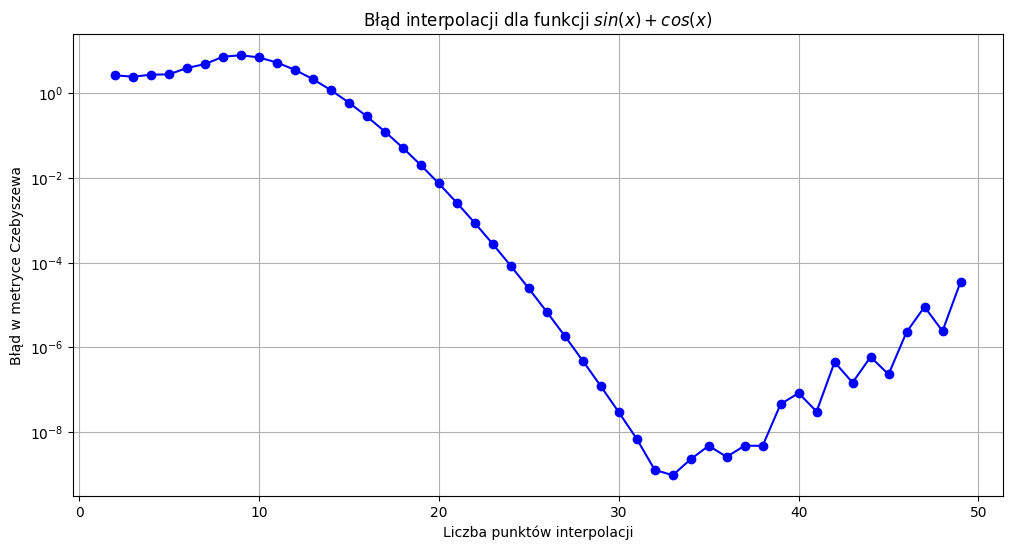
\includegraphics[width=0.8\textwidth]{wykresy/zadanie 3/tryg_blad.png}
\end{center}

\begin{minipage}{0.49\textwidth}
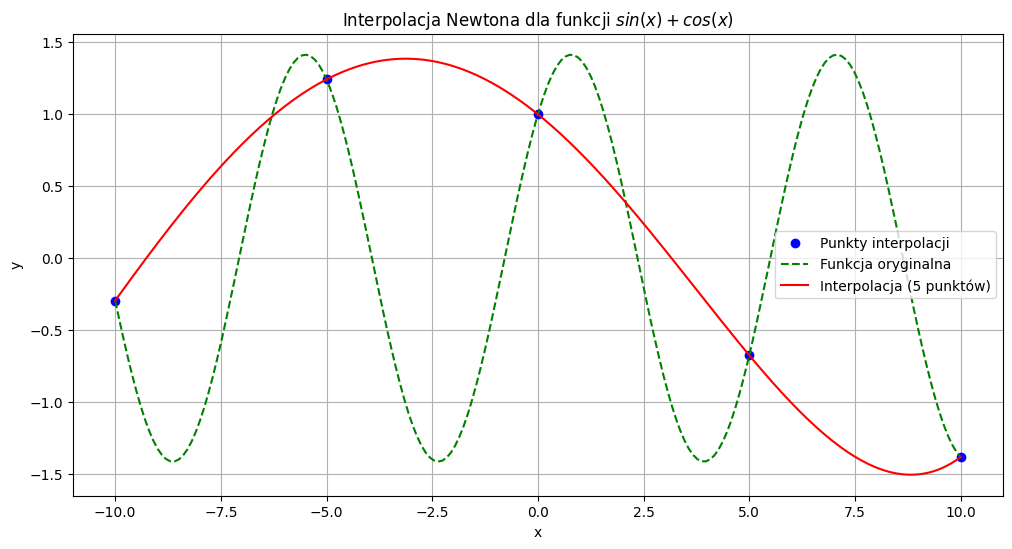
\includegraphics[width=\textwidth]{wykresy/zadanie 3/tryg_5.png}
\end{minipage}
\begin{minipage}{0.49\textwidth}
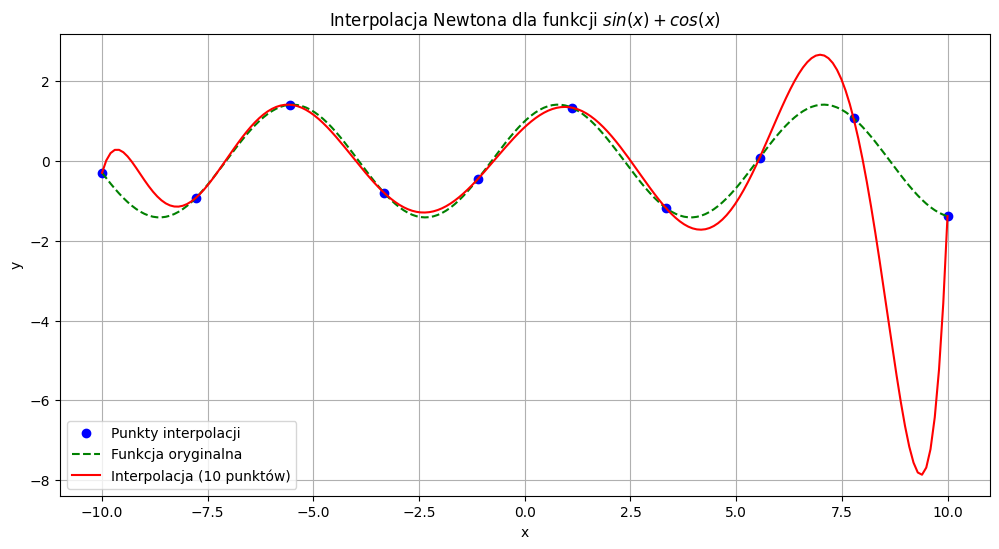
\includegraphics[width=\textwidth]{wykresy/zadanie 3/tryg_10.png}
\end{minipage}

\begin{minipage}{0.49\textwidth}
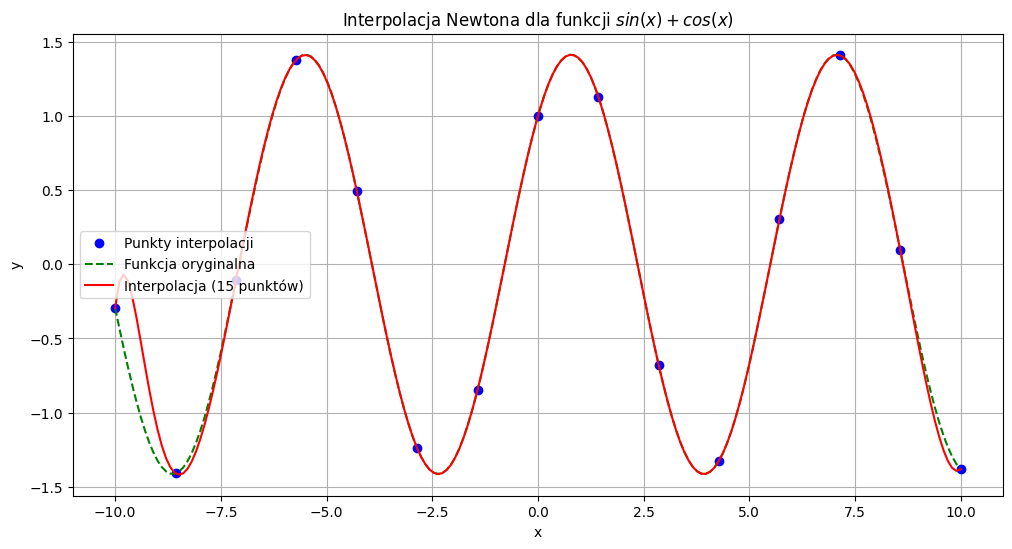
\includegraphics[width=\textwidth]{wykresy/zadanie 3/tryg_15.png}
\end{minipage}
\begin{minipage}{0.49\textwidth}
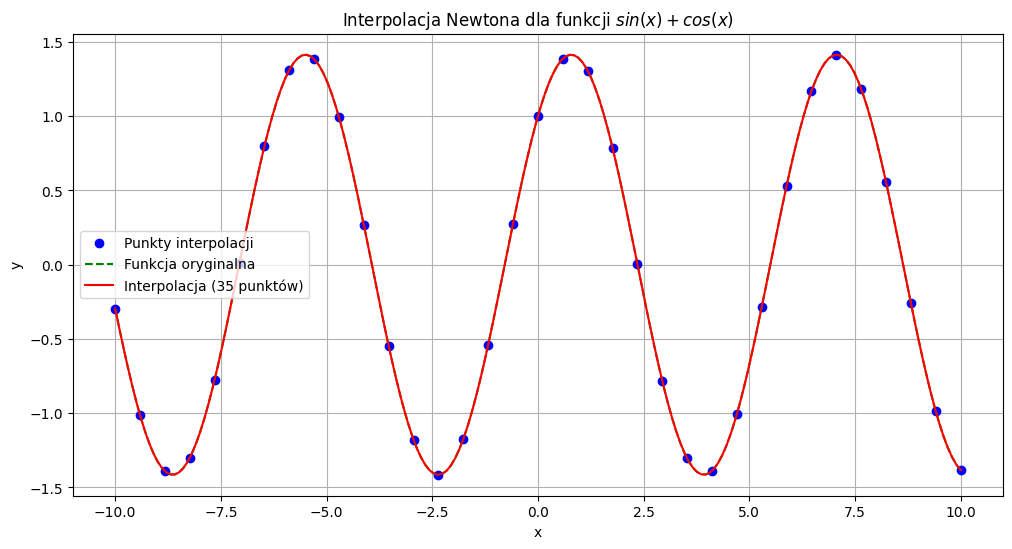
\includegraphics[width=\textwidth]{wykresy/zadanie 3/tryg_35.png}
\end{minipage}

\begin{center}
% Wykres błędów dla funkcji wymiernej
\textbf{Wyniki dla funkcji \( \frac{1}{1 + x^2} \):}  
Minimalny błąd: \( 4.78 \times 10^{-1} \)  
Osiągnięty dla 10 punktów.  
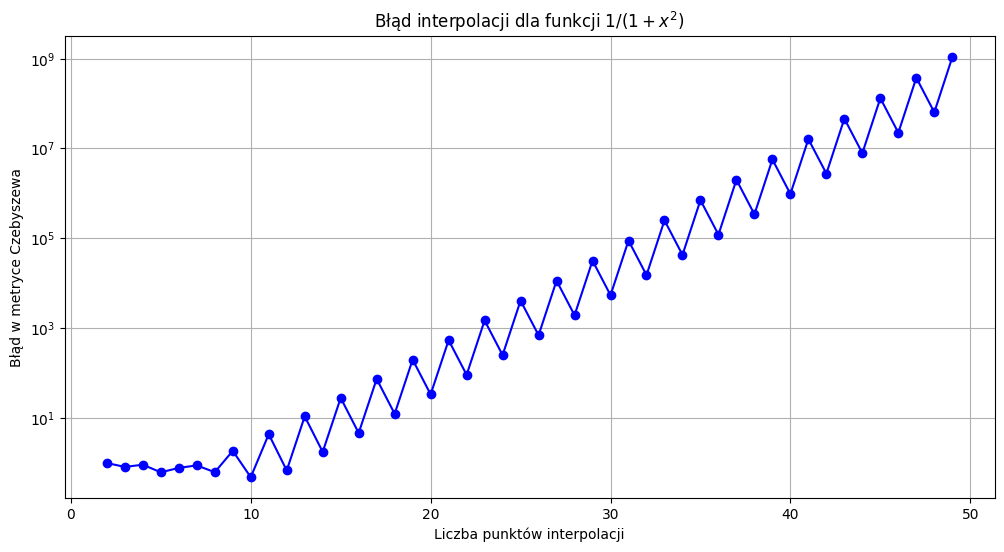
\includegraphics[width=0.8\textwidth]{wykresy/zadanie 3/wym_blad.png}
\end{center}

\begin{minipage}{0.49\textwidth}
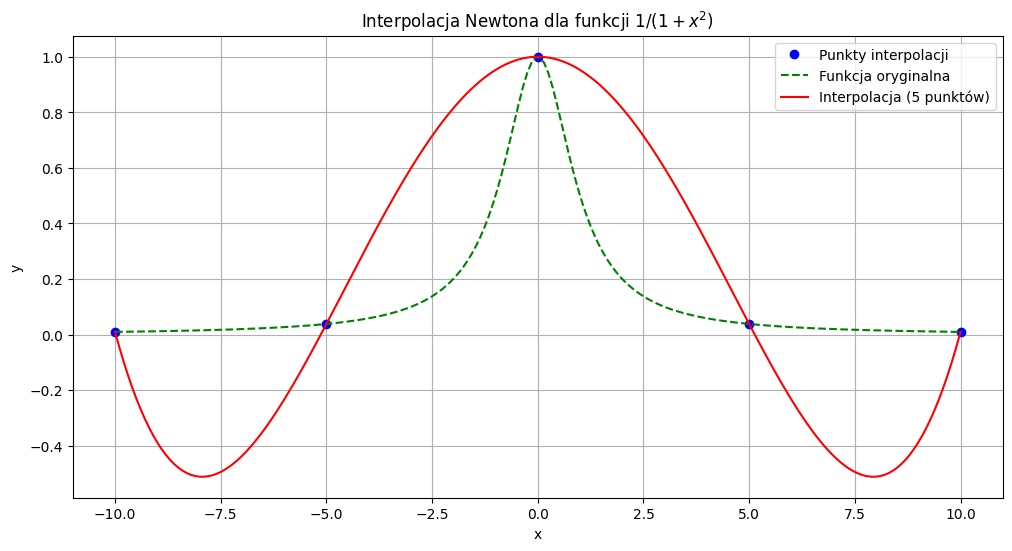
\includegraphics[width=\textwidth]{wykresy/zadanie 3/wym_5.png}
\end{minipage}
\begin{minipage}{0.49\textwidth}
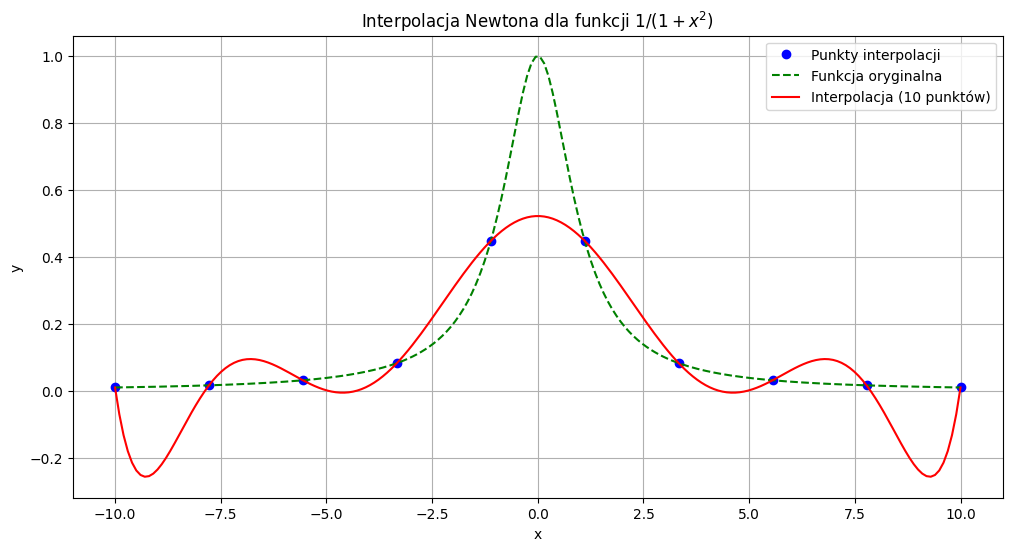
\includegraphics[width=\textwidth]{wykresy/zadanie 3/wym_10.png}
\end{minipage}

\begin{minipage}{0.49\textwidth}
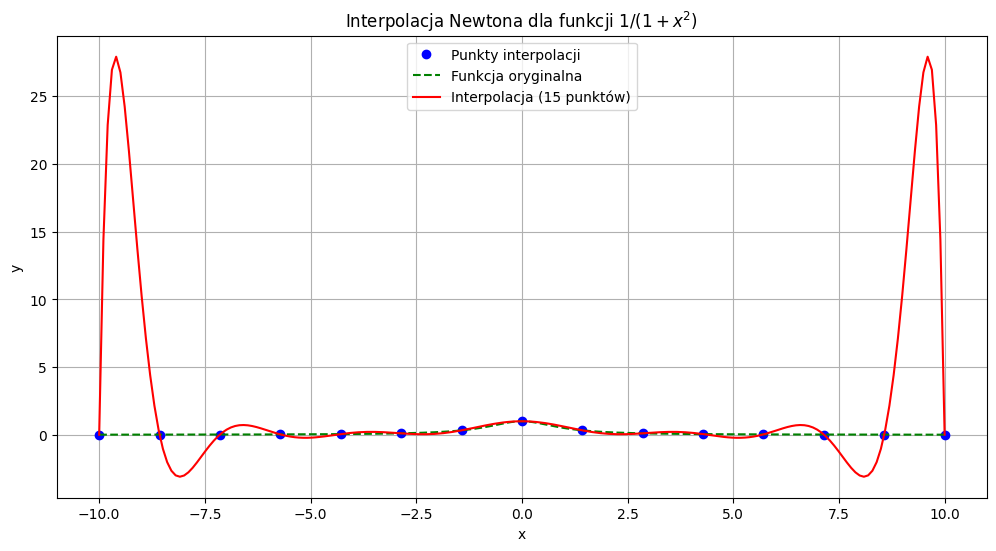
\includegraphics[width=\textwidth]{wykresy/zadanie 3/wym_15.png}
\end{minipage}
\begin{minipage}{0.49\textwidth}
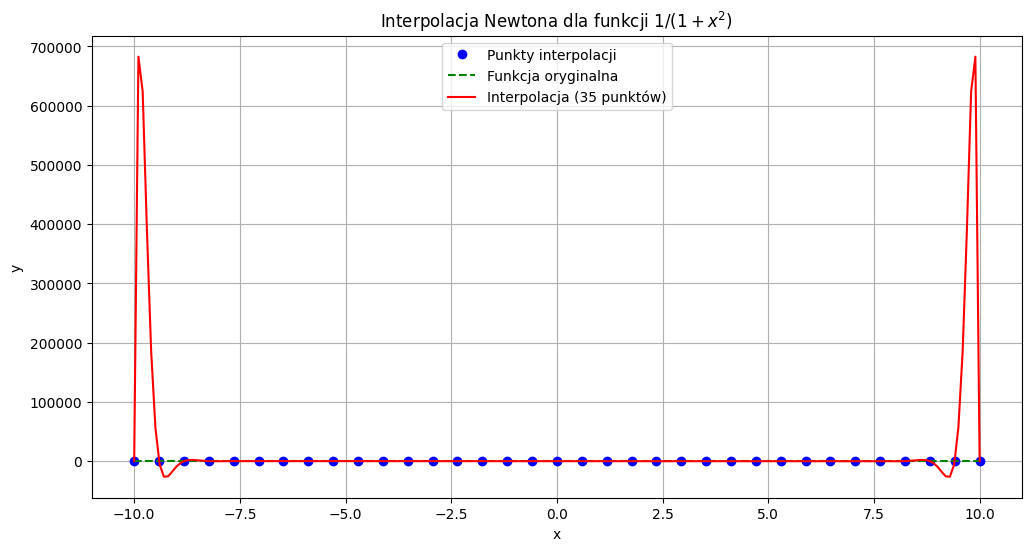
\includegraphics[width=\textwidth]{wykresy/zadanie 3/wym_35.png}
\end{minipage}

\begin{center}
% Wykres błędów dla funkcji podłoga
\textbf{Wyniki dla funkcji \( \lfloor x \rfloor \):}  
Minimalny błąd: \( 9.32 \times 10^{-1} \)  
Osiągnięty dla 20 punktów.  
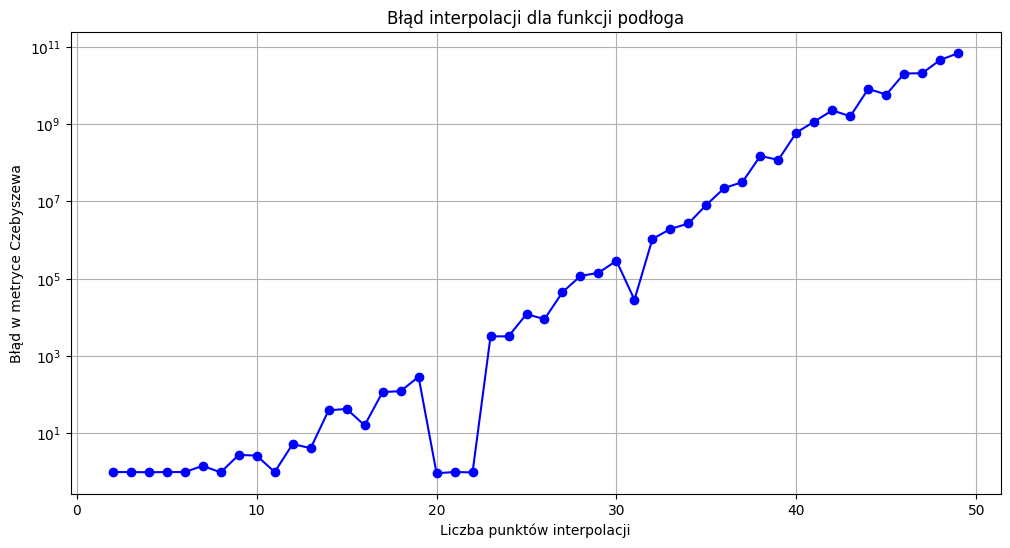
\includegraphics[width=0.8\textwidth]{wykresy/zadanie 3/floor_blad.png}
\end{center}

\begin{minipage}{0.49\textwidth}
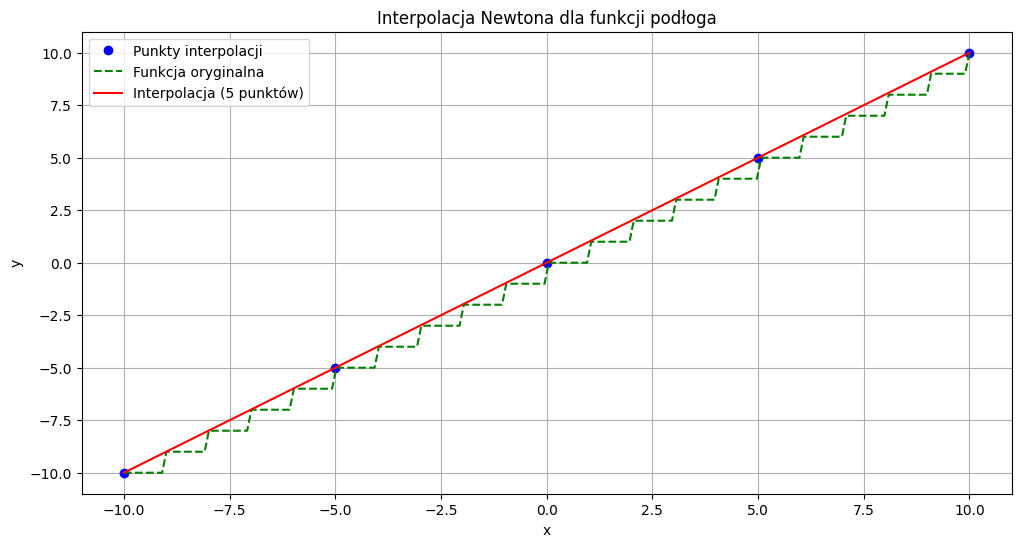
\includegraphics[width=\textwidth]{wykresy/zadanie 3/floor_5.png}
\end{minipage}
\begin{minipage}{0.49\textwidth}
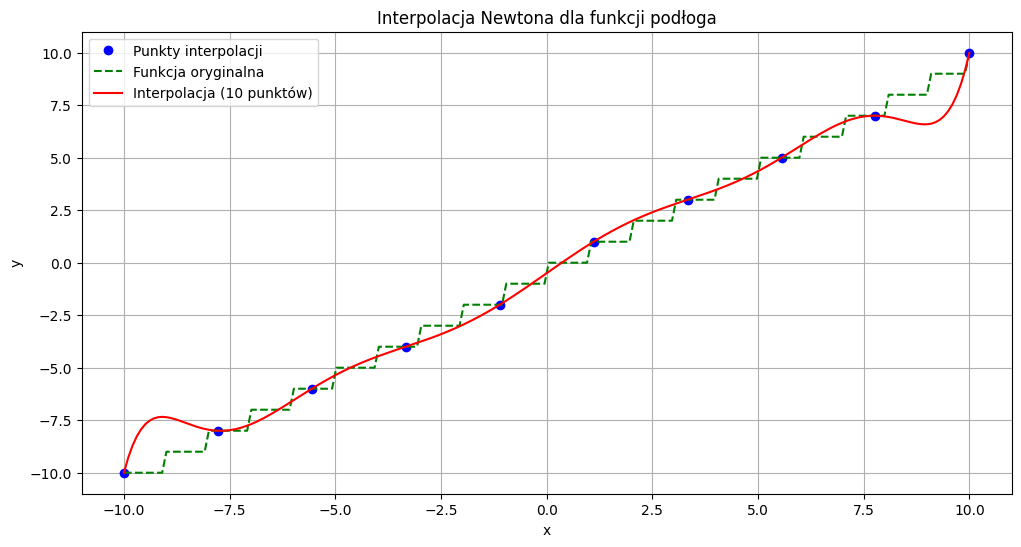
\includegraphics[width=\textwidth]{wykresy/zadanie 3/floor_10.png}
\end{minipage}

\begin{minipage}{0.49\textwidth}
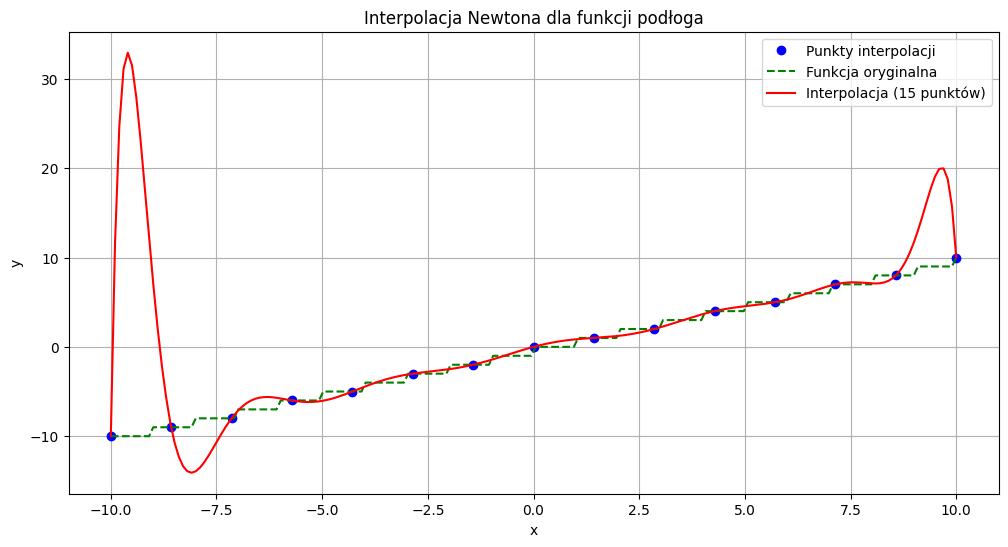
\includegraphics[width=\textwidth]{wykresy/zadanie 3/floor_15.png}
\end{minipage}
\begin{minipage}{0.49\textwidth}
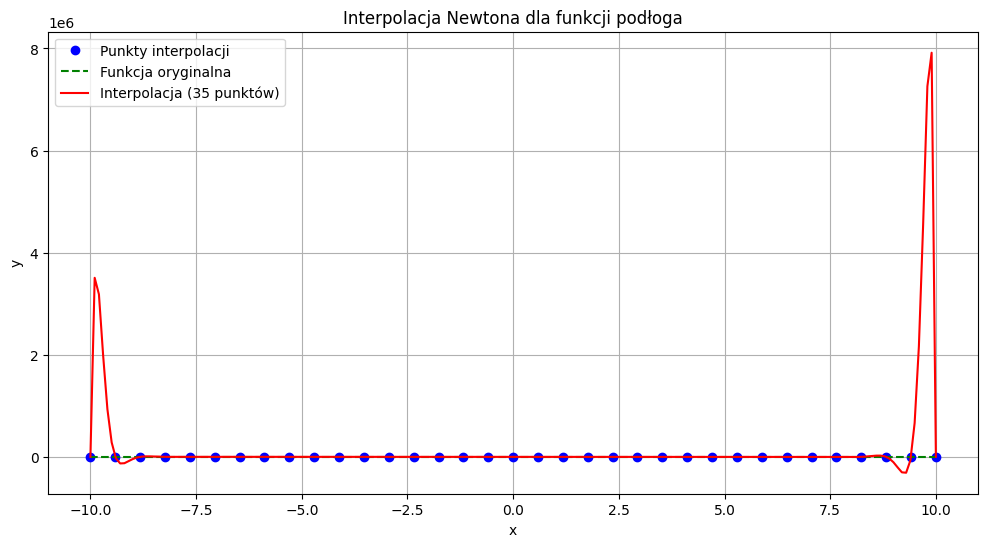
\includegraphics[width=\textwidth]{wykresy/zadanie 3/floor_35.png}
\end{minipage}

\textbf{Wnioski:}
\begin{itemize}
    \item \textbf{Efektywność przy umiarkowanej liczbie punktów:} Dodawanie dużej liczby punktów interpolacyjnych niekoniecznie poprawia wyniki. Wręcz przeciwnie, prowadzi to do większych błędów, ponieważ algorytm próbuje dopasować wielomian, co wymaga nagłych wzrostów wartości funkcji.
    \item \textbf{Trudności z funkcjami nieciągłymi:} W przypadku funkcji nieciągłych, takich jak \( \lfloor x \rfloor \), uzyskiwane błędy są znacznie większe, co wynika z problemów z dopasowaniem ciągłego wielomianu do nieciągłości.
    \item \textbf{Funkcje jednostajnie ciągłe:} Funkcje jednostajnie ciągłe, takie jak trygonometryczna i wymierna, pozwalają na uzyskanie lepszych wyników, choć nawet w tych przypadkach obserwowane są pewne ograniczenia dokładności.
    \item przy funkcjach mają wiele ekstermów widzimy charakterystyczny skoki, które wynikają z częstych zmian tempa przyrostu. 
\end{itemize}
